\section{Auswertung}
\label{sec:Auswertung}
\subsection{Frequenzverhältnisse bei einer Schwebung}
\label{sec:Frequenzverhältnisse}
Die gezählten Verhältnisse der Frequenzen lassen sich Tabelle \ref{tab:verhaeltnisse} entnehmen. Da die Grenzen der Schwebung nicht immer eindeutig ab zu lesen sind, wird eine Abweichung von $\pm1$ veranschlagt. Graphisch ergibt sich so Abb. \ref{fig:verhaeltnisse}, wobei $\omega_\pm=v_+ \pm v_-$ gilt und $C_k$ mit $3\%$ Abweichung behaftet ist.

\begin{table}
  \centering
\caption{gemessene Frequenzverhältnisse}
\label{tab:verhaeltnisse}
\sisetup{round-mode = places , round-precision = 2}
\begin{tabular}{S S}
  \toprule
  {$C_k/nF$} & {Peaks pro Schwebung}\\
  \midrule
  1.200000000000000000e+01 & 1.700000000000000000e+01\\
  9.990000000000000213e+00 & 1.400000000000000000e+01\\
  8.179999999999999716e+00 & 1.300000000000000000e+01\\
  6.860000000000000320e+00 & 1.000000000000000000e+01\\
  4.740000000000000213e+00 & 9.000000000000000000e+00\\
  2.859999999999999876e+00 & 5.000000000000000000e+00\\
  2.189999999999999947e+00 & 4.000000000000000000e+00\\
\bottomrule
\end{tabular}
\end{table}
\FloatBarrier

\begin{figure}
  \centering
  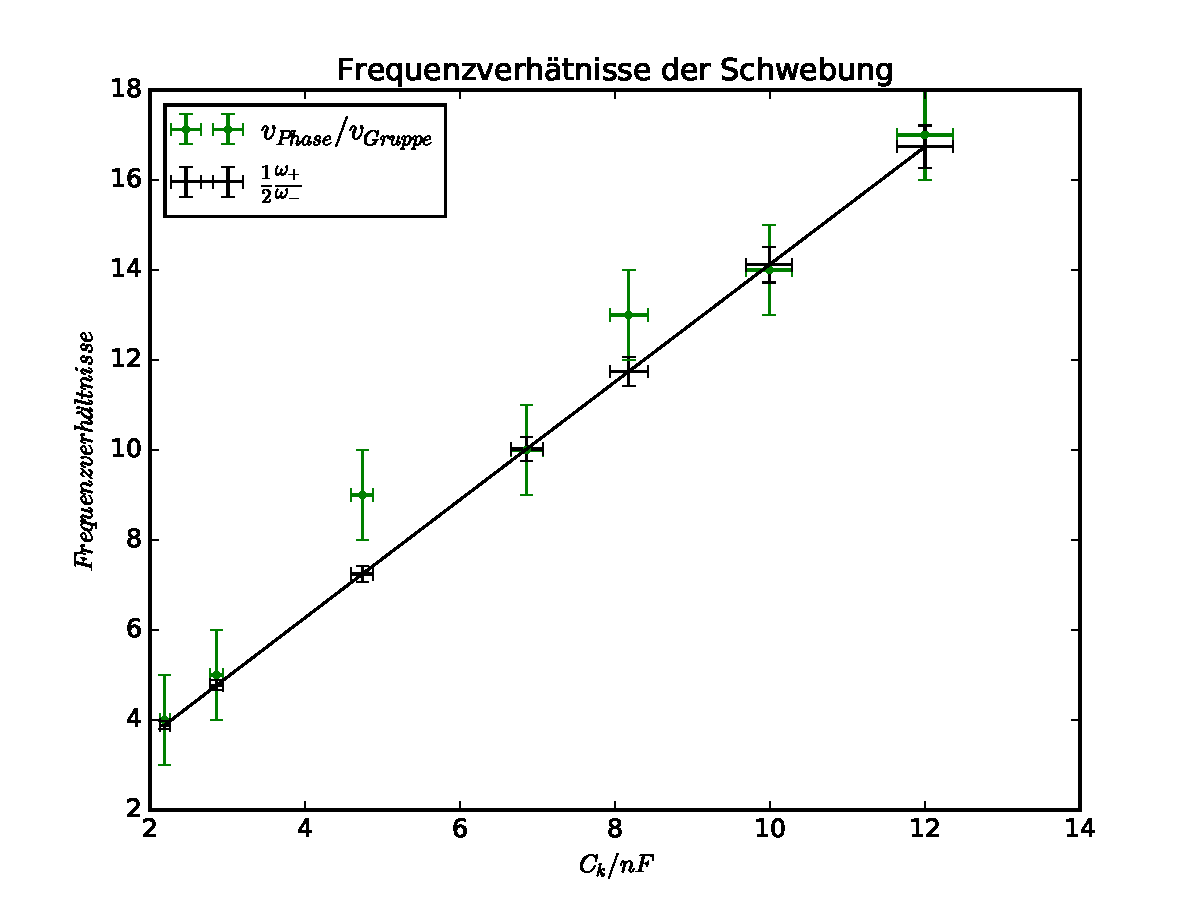
\includegraphics[width=\textwidth]{./plots/freq-ratio.pdf}
  \caption{gezählte Peaks pro Schwebung aufgetragen gegen $C_K$.}
  \label{fig:verhältnisse}
\end{figure}
\FloatBarrier

\subsection{Messung von $v_+$ und $v_-$ mittels Lissajous-Figuren}
\label{sec:Messung-v}


\begin{figure}
  \centering
  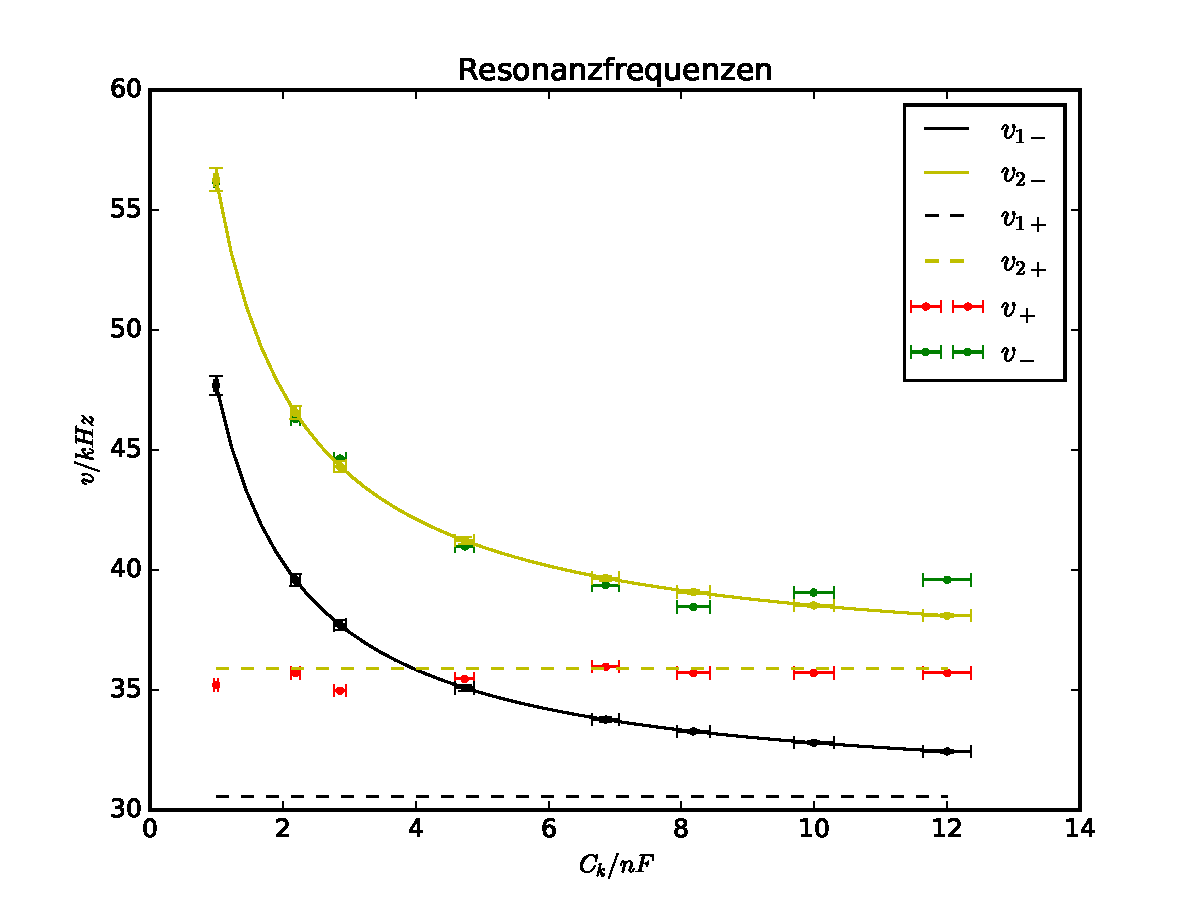
\includegraphics[width=\textwidth]{./plots/resonance.pdf}
  \caption{$v_+$ und $v_-$ aufgetragen gegen $C_K$.}
  \label{fig:frequenzen}
\end{figure}
\FloatBarrier

Die in diesem Schritt aufgenommenen Werte werden in Abb.\ref{fig:frequenzen} mit errechneten Kurven $v_{1-}$ und $v_{2-}$ für Schaltung 1 und 2. Offensichtlich wurde Schaltung 1 für die Messungen verwendet, weshalb fortan ausschließlich diese Schaltung betrachtet wird.

\begin{table}
  \centering
\caption{gemessene Resonanzfrequenzen}
\label{tab:verhaeltnisse}
\sisetup{round-mode = places , round-precision = 2}
\begin{tabular}{S S S}
  \toprule
  {$C_k/nF$} & {$\frac{v_+}{kHz}$} & {$\frac{v_-}{kHz}$}\\
  \midrule
  9.969999999999999973e-01 & 3.520000000000000284e+01 & 4.629999999999999716e+01\\
  2.189999999999999947e+00 & 3.570000000000000284e+01 & 5.617999999999999972e+01\\
  2.859999999999999876e+00 & 3.496999999999999886e+01 & 4.464000000000000057e+01\\
  4.740000000000000213e+00 & 3.546000000000000085e+01 & 4.097999999999999687e+01\\
  6.860000000000000320e+00 & 3.596999999999999886e+01 & 3.936999999999999744e+01\\
  8.179999999999999716e+00 & 3.571000000000000085e+01 & 3.846000000000000085e+01\\
  9.990000000000000213e+00 & 3.571000000000000085e+01 & 3.906000000000000227e+01\\
  1.200000000000000000e+01 & 3.571000000000000085e+01 & 3.959000000000000341e+01\\
\bottomrule
\end{tabular}
\end{table}
\FloatBarrier


\subsection{Ermittlung von $v_+$ und $v_-$ mittels Sweap-Verfahren}
\label{sec:sweap}

Da beim Sweap-Verfahren die Frequenzen nicht direkt gemessen werden, sondern nur zeitliche Abstände (zu entnehmen aus Tabelle \ref{tab:sweap}) müssen diese zunächst umgerechnet werden.

\begin{table}
  \centering
\caption{gemessene Frequenzverhältnisse}
\label{tab:sweap}
\sisetup{round-mode = places , round-precision = 2}
\begin{tabular}{S S S}
  \toprule
  {$C_k/nF$} & {$\frac{\Delta t}{ms}$} & {$\frac{\Delta t}{ms}$}\\
  \midrule
  9.969999999999999973e-01 & 4.000000000000000000e+02 & 6.480000000000000000e+02\\
  2.189999999999999947e+00 & 4.080000000000000000e+02 & 5.360000000000000000e+02\\
  2.859999999999999876e+00 & 4.000000000000000000e+02 & 5.040000000000000000e+02\\
  4.740000000000000213e+00 & 4.080000000000000000e+02 & 4.640000000000000000e+02\\
  6.860000000000000320e+00 & 4.000000000000000000e+02 & 4.400000000000000000e+02\\
  8.179999999999999716e+00 & 4.000000000000000000e+02 & 4.400000000000000000e+02\\
  9.990000000000000213e+00 & 4.080000000000000000e+02 & 4.320000000000000000e+02\\
  1.200000000000000000e+01 & 3.920000000000000000e+02 & 4.160000000000000000e+02\\
\bottomrule
\end{tabular}
\end{table}
\FloatBarrier

\begin{table}
  \centering
\caption{gemessene Frequenzverhältnisse}
\label{tab:sweap}
\sisetup{round-mode = places , round-precision = 2}
\begin{tabular}{S S S}
  \toprule
  {$C_k/nF$} & {$\frac{v_+}{kHz}$} & {$\frac{v_-}{kHz}$}\\
  \midrule
  9.969999999999999973e-01 & 3.523100000000000165e+01 & 5.511192000000000490e+01\\
  2.189999999999999947e+00 & 3.587232000000000198e+01 & 4.613344000000000733e+01\\
  2.859999999999999876e+00 & 3.523100000000000165e+01 & 4.356816000000000599e+01\\
  4.740000000000000213e+00 & 3.587232000000000198e+01 & 4.036156000000000432e+01\\
  6.860000000000000320e+00 & 3.523100000000000165e+01 & 3.843760000000000332e+01\\
  8.179999999999999716e+00 & 3.523100000000000165e+01 & 3.843760000000000332e+01\\
  9.990000000000000213e+00 & 3.587232000000000198e+01 & 3.779628000000000299e+01\\
  1.200000000000000000e+01 & 3.458968000000000131e+01 & 3.651364000000000232e+01\\

\bottomrule
\end{tabular}
\end{table}
\FloatBarrier


\begin{figure}
  \centering
  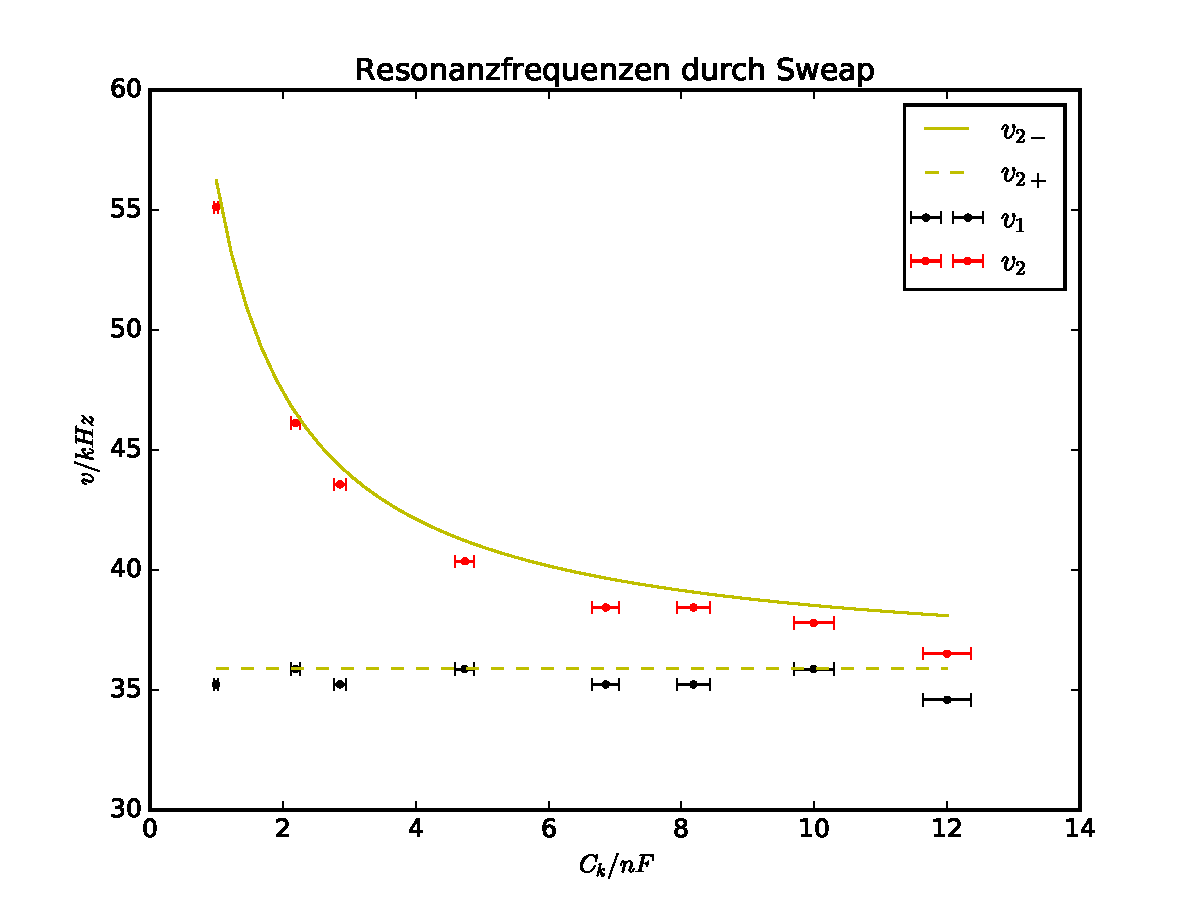
\includegraphics[width=\textwidth]{./plots/sweap.pdf}
  \caption{$v_+$ und $v_-$ aufgetragen gegen $C_K$.}
  \label{fig:sweap}
\end{figure}
\FloatBarrier
